%LTeX: language=it
\begin{figure}[H]
    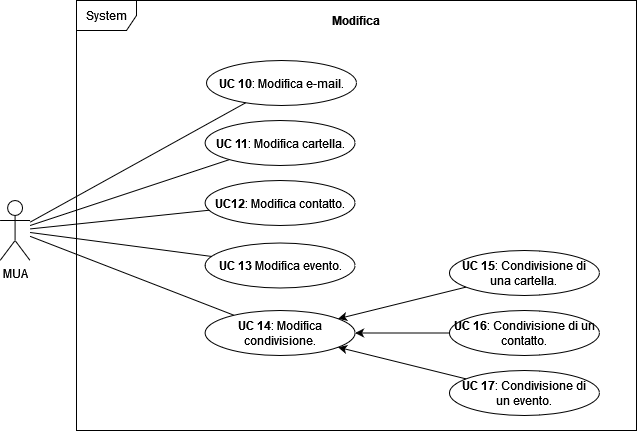
\includegraphics[width=0.75\textwidth]{sections/uc_imgs/UC-modifica.png}
    \centering
    \caption{Casi d'uso relativi alla modifica}
\end{figure}

\subsection{UC 10 - Modifica e-mail} \label{sec:UC10}
    \begin{itemize}
        \item \textbf{Attore principale}: MUA;
        \item \textbf{Descrizione}: il MUA deve poter modificare una e-mail nel sistema;
        \item \textbf{Precondizioni}: l’account che il MUA gestisce è registrato nel sistema, ha un connessione aperta con il sistema ed è autenticato;
        \item \textbf{Postcondizioni}: l'e-mail è stata modificata con successo, ed è stata salvata nel sistema;
        \item \textbf{Scenario principale}:
            \begin{enumerate}
                \item il MUA trasmette il destinatario dell'e-mail modificato (\hyperref[sec:UC10.1]{UC 10.1});
                \item il MUA trasmette il mittente dell'e-mail modificato(\hyperref[sec:UC10.2]{UC 10.2});
                \item il MUA trasmette l'oggetto dell'e-mail modificato(\hyperref[sec:UC10.3]{UC 10.3});
                \item il MUA trasmette il corpo dell'e-mail modificato(\hyperref[sec:UC10.4]{UC 10.4});
                \item il MUA trasmette la cartella di appartenenza dell'email modificata(\hyperref[sec:UC10.5]{UC 10.5});
                \item il sistema salva l'e-mail con le modifiche nel sistema.
            \end{enumerate}
        \item \textbf{Inclusioni}: nessuna;
        \item \textbf{Generalizzazioni}: nessuna;
        \item \textbf{Estensioni}: 
            \begin{enumerate}[label=\alph*.]
                \item il sistema non riesce a modificare l'e-mail perchè l'email ha troppe cartelle di destinazione:
                \begin{enumerate}[label=\arabic*.]
                    \item il sistema ritorna un errore al MUA di troppe cartelle (\hyperref[sec:UC10.6]{UC 10.6}).
                \end{enumerate}
            \end{enumerate}
    \end{itemize}

    \begin{figure}[H]
        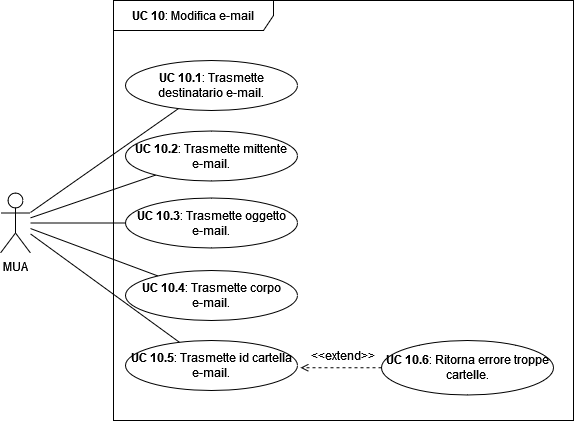
\includegraphics[width=0.85\textwidth]{sections/uc_imgs/UC10.png}
        \centering
        \caption{Diagramma sotto-casi UC 10}
    \end{figure}

    \subsubsection{UC 10.1 - Trasmette destinatario e-mail} \label{sec:UC10.1}
    \begin{itemize}
        \item \textbf{Attore}: MUA;
        \item \textbf{Descrizione}: il MUA invia al sistema il nuovo destinatario dell'e-mail;
        \item \textbf{Precondizioni}: il MUA sta usando la funzionalità di modifica di un'e-mail;
        \item \textbf{Postcondizioni}: il sistema conosce il nuovo indirizzo di posta elettronica del destinatario dell'e-mail;
        \item \textbf{Scenario principale}:
            \begin{enumerate}
                \item il MUA trasmette il destinatario modificato;
            \end{enumerate}
        \item \textbf{Inclusioni}: nessuna;
        \item \textbf{Generalizzazioni}: nessuna;
        \item \textbf{Estensioni}: nessuna;
    \end{itemize}

    \subsubsection{UC 10.2 - Trasmette mittente e-mail} \label{sec:UC10.2}
    \begin{itemize}
        \item \textbf{Attore}: MUA;
        \item \textbf{Descrizione}: il MUA invia al sistema il nuovo mittente dell'e-mail;
        \item \textbf{Precondizioni}: il MUA sta usando la funzionalità di modifica di un'e-mail;
        \item \textbf{Postcondizioni}: il sistema conosce il nuovo indirizzo di posta elettronica del mittente dell'e-mail;
        \item \textbf{Scenario principale}:
            \begin{enumerate}
                \item il MUA trasmette il mittente modificato;
            \end{enumerate}
        \item \textbf{Inclusioni}: nessuna;
        \item \textbf{Generalizzazioni}: nessuna;
        \item \textbf{Estensioni}: nessuna.
    \end{itemize}

    \subsubsection{UC 10.3 - Trasmette oggetto e-mail} \label{sec:UC10.3}
    \begin{itemize}
        \item \textbf{Attore}: MUA;
        \item \textbf{Descrizione}: il MUA invia al sistema il nuovo oggetto dell'e-mail;
        \item \textbf{Precondizioni}: il MUA sta usando la funzionalità di modifica di un'e-mail;
        \item \textbf{Postcondizioni}: il sistema conosce il nuovo oggetto dell'e-mail;
        \item \textbf{Scenario principale}:
            \begin{enumerate}
                \item il MUA trasmette l'oggetto dell'e-mail modificato;
            \end{enumerate}
        \item \textbf{Inclusioni}: nessuna;
        \item \textbf{Generalizzazioni}: nessuna;
        \item \textbf{Estensioni}: nessuna.
    \end{itemize}

    \subsubsection{UC 10.4 - Trasmette corpo e-mail} \label{sec:UC10.4}
    \begin{itemize}
        \item \textbf{Attore}: MUA;
        \item \textbf{Descrizione}: il MUA invia al sistema il nuovo corpo dell'e-mail;
        \item \textbf{Precondizioni}: il MUA sta usando la funzionalità di modifica di un'e-mail;
        \item \textbf{Postcondizioni}: il sistema conosce il nuovo corpo dell'e-mail;
        \item \textbf{Scenario principale}:
            \begin{enumerate}
                \item il MUA trasmette il corpo dell'e-mail modificato;
            \end{enumerate}
        \item \textbf{Inclusioni}: nessuna;
        \item \textbf{Generalizzazioni}: nessuna;
        \item \textbf{Estensioni}: nessuna.
    \end{itemize}

    \subsubsection{UC 10.5 - Trasmette id cartella e-mail} \label{sec:UC10.5}
    \begin{itemize}
        \item \textbf{Attore}: MUA;
        \item \textbf{Descrizione}: il MUA invia al sistema il nuovo id della cartella di destinazione dell'e-mail;
        \item \textbf{Precondizioni}: il MUA sta usando la funzionalità di modifica di un'e-mail;
        \item \textbf{Postcondizioni}: il sistema conosce la nuova cartella di destinazione dell'e-mail;
        \item \textbf{Scenario principale}:
            \begin{enumerate}
                \item il MUA trasmette l'id della cartella di destinazione dell'e-mail modificato;
            \end{enumerate}
        \item \textbf{Inclusioni}: nessuna;
        \item \textbf{Generalizzazioni}: nessuna;
        \item \textbf{Estensioni}:             
        \begin{enumerate}[label=\alph*.]
            \item il sistema non riesce a modificare l'e-mail perchè ci sono troppe cartelle di destinazione in cui salvare l'email:
            \begin{enumerate}[label=\arabic*.]
                \item il sistema ritorna un errore al MUA di troppe cartelle (\hyperref[sec:UC10.6]{UC 10.6}).
            \end{enumerate}
        \end{enumerate}
    \end{itemize}

    \subsubsection{UC 10.6 - Ritorna errore troppe cartelle} \label{sec:UC10.6}
    \begin{itemize}
        \item \textbf{Attore}: MUA;
        \item \textbf{Descrizione}: il MUA riceve l'errore che le cartelle di destinazione dell'email sono troppe;
        \item \textbf{Precondizioni}: il MUA ha trasmesso le cartelle di destinazione e-mail;
        \item \textbf{Postcondizioni}: il MUA viene notificato che le cartelle sono troppe;
        \item \textbf{Scenario principale}:
            \begin{enumerate}
                \item il sistema verifica il numero di cartelle;
                \item il sistema rileva che il numero di cartelle supera la soglia massima consentita;
                \item il sistema non modifica l'email e notifica il MUA dell'eccesso di cartelle nella e-mail;
            \end{enumerate}
        \item \textbf{Inclusioni}: nessuna;
        \item \textbf{Generalizzazioni}: nessuna;
        \item \textbf{Estensioni}: nessuna.
    \end{itemize}
